\chapter{Konzepte der Informatik: Bausteine von Algorithmen}

Mit den digitalen Pins, die sich als Ausgänge und Eingänge nutzen lassen, lassen sich zahlreiche Projekte umsetzen. Allerdings wird die Programmierung schnell unübersichtlich oder unnötig aufwendig, wenn man sich nicht mit algorithmischen Strukturen auskennt. Daher geht es im folgenden Kapitel um die Einführung von grundlegenden algorithmischen Bausteinen.

\bigskip
In diesem Kapitel lernst du\dots
\begin{itemize}
	\item \dots Variablen zu benutzen,
	\item \dots mit Schleifen effizient zu programmieren,
	\item \dots zufällige Ereignisse zu programmieren,
	\item \dots den Arduino mit dem Computer kommunizieren zu lassen,
	\item \dots überblicksweise, wie die USB-Verbindung funktioniert,
	\item \dots was es mit den berühmten Einsen und Nullen auf sich hat,
	\item \dots wie man Programme zur Planung oder zum Vergleich auf Papier einfach darstellen kann.
\end{itemize}

\bigskip

\begin{projektueberblick}
	\item Auto-Blinker \dotfill \pageref{proj:blinker}
	\item Bombe bauen \dotfill \pageref{proj:bombe}
	\item Reaktionszeitmesser \dotfill \pageref{proj:reaktionszeitmesser}
\end{projektueberblick}

\newpage
\section{Programme mit Variablen strukturieren}
% Variablen strukturieren Programme: Vergleich von Programm mit und ohne Variablen
% -> Vorstellung als Koffer; Zeichnung mit Verweis auf Speicherfläche
% -> sinnvolle Benennung von Variablen
\vspace{-0.5\baselineskip}
\begin{aufgabe}
	Jonas und Jana haben jeweils LEDs an die Pins 13 bis 11 angeschlossen und steuern diese mit den unten abgebildeten Programmen. Vergleiche die beiden Programme im Hinblick auf ihre Wirkung und die Art der Programmierung. Welches gefällt dir besser?
	
	Zusatzüberlegung: Wie viel muss man ändern, wenn man zum Beispiel Probleme mit Pin 13 hat und deshalb die zugehörige LED an Pin 10 anschließen will?
\end{aufgabe}
\marginpar{%
	\textattachfile[description={Folie zu Kap. \thechapter, Variableneinsatz}]{./Auftraege/kap4-auftrag-variablen.pdf}{%
		\footnotesize\folie Folie %
	}%
	\footnotesize%
	%\folie \href{run:./Auftraege/kap4-auftrag-variablen.pdf}{Folie}\\%
	\\öffnen%
}

\vspace{-0.75\baselineskip}
\begin{figure}[H]
	\begin{minipage}{0.48\textwidth}
		\centering
		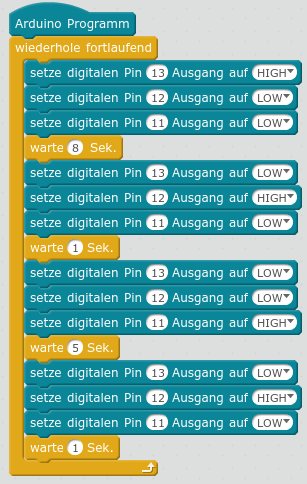
\includegraphics[width=0.75\textwidth]{pics/ampel-ohne-variablen.png}
		\caption{Jonas Programm zum Steuern der LEDs.}
	\end{minipage}
	\hfill
	\begin{minipage}{0.48\textwidth}
		\centering
		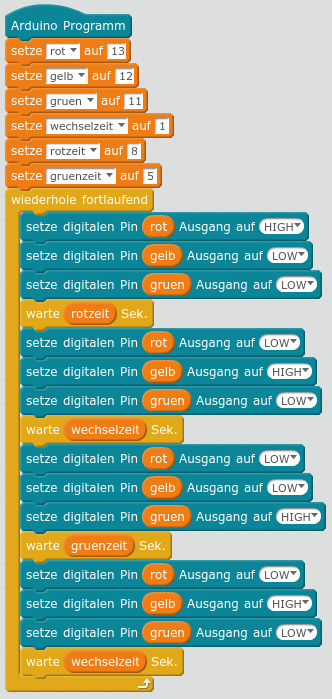
\includegraphics[width=0.75\textwidth]{pics/ampel-mit-variablen.png}
		\caption{Janas Programm zum Steuern der LEDs.}
	\end{minipage}
\end{figure}
\vspace{-0.75\baselineskip}

\begin{zsfg}{Variablen}
	\begin{wrapfigure}{r}{0.25\textwidth}
		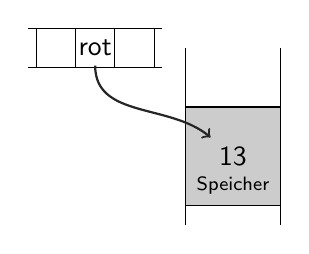
\begin{tikzpicture}[scale=0.5]
		\draw (-0.2,0) -- (3.2,0);
		\draw (-0.2,1) -- (3.2,1);
		\draw [fill=white] (0,0) rectangle (1,1);
		\draw [fill=white] (1,0) rectangle (2,1);
		\draw [fill=white] (2,0) rectangle (3,1);
		\node (rot) at (1.5,0.5) {\sffamily rot};
		\draw (3.8,0.5) -- (3.8,-4);
		\draw (6.2,0.5) -- (6.2,-4);
		\draw [fill=gray!40] (3.8,-1) rectangle (6.2,-3.5);
		\node (wert) at (5,-2.25) {\sffamily 13};
		\draw [gray!30!black, thick,->] (rot) to [out=270,in=140] (wert);
		\node at (5,-3) {\sffamily\scriptsize Speicher};
		\end{tikzpicture}
	\end{wrapfigure}
	Eine Variable kann man sich als Koffer vorstellen, der einen Namen bekommt und in dem man einen Zahlenwert oder ein Wort speichert. Jedes Mal, wenn der Name des Koffers aufgerufen wird, wird der abgespeicherte Wert hervorgeholt und an die Stelle des Namens gesetzt.	
	Intern wird der Variablenname als Verweis auf einen bestimmten Speicherplatz genutzt, in dem der Wert der Variable abgelegt ist.
	
	Wir unterscheiden drei \textbf{Datentypen}, die in Variablen abgespeichert werden: Zahlen (runde Felder), Zeichen (rechteckige Felder) und Wahrheitswerte (spitze Felder: Wahr oder falsch). Wahrheitswerte werden auch \emph{boolsche Variablen} genannt.
\end{zsfg}

% Variablen:
% die beiden Programme von Jonas und Jana bewirken das Gleiche (Ampelschaltung)
% Jonas Programm ist kürzer
% Janas Programm ist verständlicher, weil sie Variablen einsetzt, deren Name die Funktion verdeutlicht
% Janas Programm ist praktischer, weil man bei einer Änderung eines Pins oder einer Pause das Programm nur an einer Stelle ändern muss

\section{Lauflichter effizient programmieren}

Lauflichter findet man inzwischen überall in unserer Welt: An den Rändern von Landebahnen an Flughäfen, an Spieleautomaten, aufdringlichen Werbeschildern, als Blinker von modernen Autos und vieles mehr.

\begin{ziel}
	\textbf{Ziel:} Ein Auto-Blinker soll auf möglichst effiziente Weise programmiert werden.
\end{ziel}

\begin{aufgabe}
	Fange mit einem einfachen Lauflicht an und baue dieses immer weiter aus.
	\begin{enumerate}[label=\alph*), itemsep=0ex, parsep=0ex]
		\item Bringe vier LEDs mit Vorwiderständen von $330\,\Omega$ an den Pins 10 bis 13 an. Programmiere sie so, dass sie nacheinander aufleuchten und wieder ausgehen. Nutze für die Pausenzeit eine Variable.
	\end{enumerate}
	\begin{minipage}{0.76\textwidth}
		\begin{enumerate}[label=\alph*), itemsep=0ex, parsep=0ex,start=2]
			\item Du wirst leicht erkennen, dass sich die Schritte zum Aufleuchten und Ausstellen bei jeder LED wiederholen. Sie lassen sich effizienter mit einer Wiederholungsschleife programmieren, die aber nicht unendlich lange weiterläuft. 
			
			Lege eine Laufvariable namens \button{pin} an, die für die Angabe des Pins genutzt wird, der an bzw. ausgestellt werden soll. In jedem Schleifendurchlauf muss die \button{pin}-Variable dann entsprechend geändert werden.
			
			Programmiere das Lauflicht aus a) mithilfe einer Laufvariable und einer Wiederholungsschleife möglichst effizient.
		\end{enumerate}
	\end{minipage}
	\hfill
	\begin{minipage}{0.22\textwidth}
		\begin{figure}[H]
			\centering
			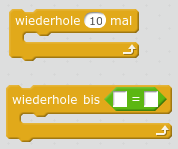
\includegraphics[width=\textwidth]{pics/schleifenvarianten.png}
			\caption{Mögliche Schleifen für Teil b.}
		\end{figure}
	\end{minipage}
	\marginpar{%
		\textattachfile[description={Arbeitsblatt zu Kap. \thechapter, Trace-Tabelle}]{./Auftraege/kap4-trace-tabelle.pdf}{%
		\ausrufezeichen%
		}%
		\footnotesize%
		%\ausrufezeichen 
		\\Trace-Tabelle
	}
	\begin{enumerate}[label=\alph*), itemsep=0ex, parsep=0ex,start=3]
		\item \emph{Für Schnelle:} Ergänze weitere LEDs und passe dein Programm daran an.
	\end{enumerate}
\end{aufgabe}

\begin{aufgabe}
	Programmiere ein Lauflicht, das hin- und zurückläuft.
\end{aufgabe}

\marginpar{%
	\footnotesize%
	\video \\
	\href{https://www.youtube.com/watch?v=s317_5aFL6E}{Blinker-Beispielvideo}
}
\begin{projekt}[Auto-Blinker]\label{proj:blinker}
	Programmiere ein Lauflicht so, wie es auch als Blinker in modernen Autos genutzt wird.
\end{projekt}

\begin{zsfg}{Schleifen}
	
	Bei der Programmierung werden häufig Schleifen genutzt, die die Anweisungen in ihrem Rumpf (oder Körper) solange wiederholen, bis eine gewisse Abbruchbedingung eintritt.
	
	\emph{Zählschleifen} wiederholen die Anweisungen im Rumpf für eine festgelegte Anzahl von Wiederholungen.
	
	Die \texttt{wiederhole bis}-Schleife wiederholt die Anweisungen solange, bis die angegebene Bedingung wahr ist. Zum Beispiel lässt sich mit dem grünen Block für den Vergleich zweier Zahlen eine \texttt{WAHR}/\texttt{FALSCH}-Aussage erzeugen, wie man an der eckigen Form erkennt. Ein weiteres Beispiel ist der Block \texttt{lese digitalen Pin}, der ebenfalls eine \texttt{WAHR}/\texttt{FALSCH}-Aussage erzeugt (vgl. S.\,\pageref{sec:digitalread}). Die Überprüfung, ob die Bedingung wahr ist, erfolgt hier \emph{vor} der Ausführung der Befehle im Rumpf. Daher nennt man die Schleife auch \emph{kopfgesteuert}.
\end{zsfg}

\newpage
\section{Zufällige Ereignisse programmieren}

\begin{wrapfigure}{r}{0.2\textwidth}
	\centering
	
\includegraphics[width=0.18\textwidth]{pics/zufallszahl.png}
\end{wrapfigure}
Viele Dinge werden interessanter, wenn sie sich nicht immer auf die genau gleiche Art wiederholen. Für diese Fälle kann man im Programm den grünen Block für Zufallszahlen verwenden, der jedes Mal eine neue Zufallszahl erzeugt, wenn er aufgerufen wird. Ein einfaches Beispiel ist die \enquote{Bombe}, die man bei dem Spiel \enquote{Tick Tack Bumm} startet und die man so lange herum geben muss, bis sie explodiert. Dabei ist die Dauer des Tickens ein zufälliger Wert zwischen ca. 5\,s und 20\,s.
\marginpar{%
	\footnotesize%
	\video \\
	\href{https://el-voss.de/downloads/ticktack.html}{Bomben-Beispielvideo}
}
\marginpar{%
	\footnotesize%
	\textattachfile[description={Arbeitsblatt zu Kap. \thechapter, Bombenprogramm}]{./Auftraege/kap4-bombenvergleich.pdf}{
	\footnotesize%
	\ausrufezeichen}%
	\\Programm-%
	\\vergleich
}

\medskip
\begin{projekt}[Bombe bauen]\label{proj:bombe}
	Baue und programmiere eine \enquote{Bombe}, die für eine zufällige Dauer zwischen 5\,s und 20\,s tickt und dann explodiert. Die Bombe wird über einen Taster aktiviert.
\end{projekt}
\vspace{-\baselineskip}

\section{Kommunikation mit dem Arduino: Der serielle Monitor}
\label{sec:seriellermonitor}
%Reaktionszeitmesser mit Zufallselement; Aufgabe: Struktogramm
Bisher hatte die Kommunikation mit dem Arduino stets nur eine Richtung: Vom Computer zum Arduino. Das reicht nicht mehr, wenn der Arduino etwas messen und dem Anwender dann mitteilen soll, was er gemessen hat. Für solche Fälle ist der serielle Monitor die einfachste Kommunikationsmöglichkeit zwischen Arduino und Computer.

\begin{ziel}
	\textbf{Frage:} Wie kann der Arduino mit dem Computer kommunizieren?
\end{ziel}

\begin{wrapfigure}{r}{0.25\textwidth}
	\centering
	
\includegraphics[width=0.23\textwidth]{pics/serialprint.png}
\end{wrapfigure}
Mit dem Block \button{Sende Text an seriellen Port} kann der Arduino angewiesen werden, den eingegebenen Text über die serielle Schnittstelle an den Computer zu senden. Der Text kann auch eine Zahl sein - diese Zahl wird dann eben nicht mehr als Zahl, sondern als Text behandelt und ausgegeben. Am Computer sieht man das Ergebnis im Fenster unten rechts, in dem bisher bereits Statusnachrichten zur Übertragung des Programms auf den Arduino zu sehen waren. \emph{Hier muss der Zeichenmodus eingestellt werden, damit die Daten für uns lesbar sind.}

\begin{projekt}[Reaktionszeitmesser]\label{proj:reaktionszeitmesser}
	Baue und programmiere einen Reaktionszeitmesser.
	
	\begin{wrapfigure}{r}{0.2\textwidth}
		\centering
		
\includegraphics[width=0.18\textwidth]{pics/stoppuhr.png}
	\end{wrapfigure}
	Der Reaktionszeitmesser soll zunächst warten, bis ein Taster gedrückt wurde, der besagt, dass es losgehen kann. Dann wird eine LED angeschaltet (Vorwiderstand!) und nach einer zufälligen Zeit wieder ausgeschaltet. Nun beginnt die Zeitmessung. Die Stoppuhr läuft solange, bis der Taster gedrückt wurde. Die gemessene Zeit wird dann über den seriellen Monitor ausgegeben und es wird erneut gewartet, bis der Anwender bestätigt, dass es losgehen kann.
	
	Miss mindestens zehn Mal deine Reaktionszeit und bestimme den Mittelwert. Bist du besser als dein Partner?
	
	\emph{Für Schnelle:} Nutze den \button{Verbinde <\_> mit <\_>}-Block, um der Ausgabe folgende Form zu geben: \enquote{Deine Reaktionszeit: 10s}.
	
	{\scriptsize Idee: Frick, Fritsch und Trick (2015): \emph{Einführung in Mikrocontroller - Der Arduino als Steuerzentrale}, Bad Saulgau}
\end{projekt}

\begin{zsfg}{Serielle Schnittstellen}
	
	\begin{wrapfigure}{r}{0.5\textwidth}
		\centering
		\begin{tikzpicture}[scale=0.5]
		\fill [white] (-4,-0.7) rectangle (8,3.2);
		\foreach \x in {1,...,7} \draw [dashed] (\x,-0.5) -- (\x,2.5);
		\draw (0,0) -- (1,0) -- (1,2) -- (2,2) -- (2,0) -- (3,0) -- (3,2) -- (6,2) -- (6,0) -- (8,0);
		\foreach \b in {0,2,6,7} \node at (\b+0.5,-0.4) {\sffamily\scriptsize 0};
		\foreach \b in {1,3,4,5} \node at (\b+0.5,-0.4) {\sffamily\scriptsize 1};
		\draw [{<[length=3pt, width=5pt]}-{>[length=3pt, width=5pt]}] (1,2.2) -- (2,2.2) node at (1.5,2.7) {\sffamily\scriptsize $8,68\,\mu s$};
		\node at (-2,0) {\sffamily \scriptsize logisch 0 / 0\,V};
		\node at (-2,2) {\sffamily \scriptsize logisch 1 / 5\,V};
		\end{tikzpicture}
		\caption{Durch ein gepulstes elektrisches Potential wird eine Folge von Bits zwischen Arduino und Computer übertragen.}
		\vspace{-\baselineskip}
	\end{wrapfigure}
	Bei seriellen Schnittstellen werden die Bits, also die Einsen und Nullen nacheinander (seriell) von einem Gerät zum nächsten geschickt. Dazu werden el. Potenzialpulse mit einer festgelegten Länge von einem Gerät gesendet und vom anderen Gerät empfangen. Dabei kann ein Puls mit 5V als eine 1 und ein Puls von 0V als eine 0 interpretiert werden. In unserem Fall ist eine Bitrate von 115200 Bit pro Sekunde festgelegt, wodurch ein Bit bzw. Potenzialpuls $\SI{8,68}{\micro\second}$ dauert.
	
	\begin{wrapfigure}{r}{0.3\textwidth}
		\centering
		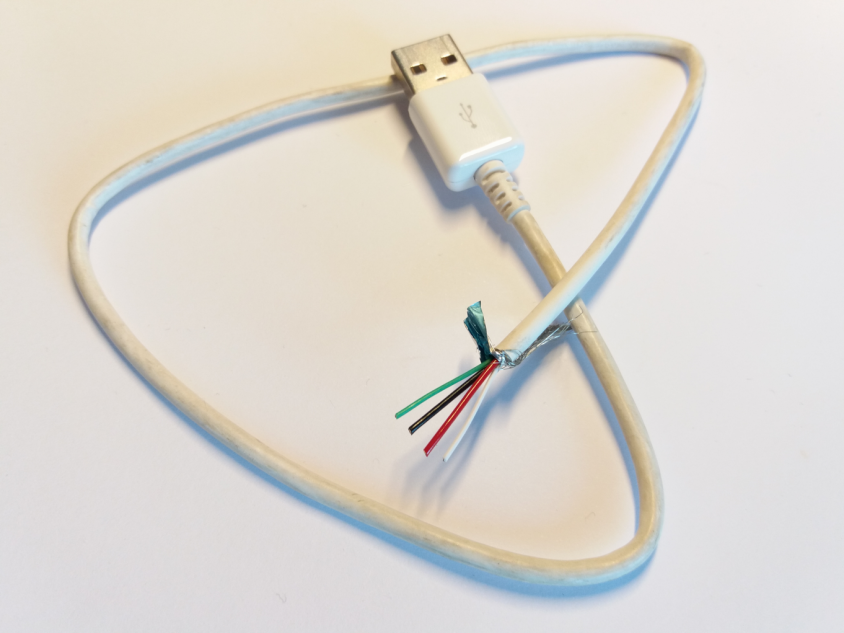
\includegraphics[width=0.3\textwidth]{pics/usbkabel-qn.png}
		\caption{Ein USB-Kabel enthält vier Leitungen.}
		\vspace{-\baselineskip}
	\end{wrapfigure}
	Die bekannteste serielle Schnittstelle ist USB - der \emph{Universal Serial Bus}. Für die Kommunikation werden vier Kabel benötigt, die man erkennen kann, wenn man das USB-Kabel durchschneidet: Das schwarze Kabel (GND) und das rote Kabel (5\,V) stellen die Spannungsversorgung sicher. Dazu kommt eine Empfängerleitung (RX) und eine Senderleitung (TX). Der Empfängerpin des Arduino ist Pin 0 und muss mit dem Senderpin am Computer verbunden sein. Umgekehrt muss der Senderpin des Arduino (Pin 1) mit dem Empfängerpin am Computer verbunden sein. Wenn etwas an Pin 0 oder 1 des Arduino angeschlossen ist, kann es passieren, dass die Übertragung eines neuen Programms auf den Arduino nicht funktioniert, weil das angeschlossene Bauteil das richtige Setzen der Potentialpulse verhindert.
\end{zsfg}

\begin{aufgabe}
	Angenommen, du hast ein Programm erstellt, das 75\,kB groß ist. Berechne, wie lange es bei einer Bitrate von 115200 Bit pro Sekunde dauert, diese Datenmenge auf den Arduino zu übertragen.
	
	\emph{Hinweise:} 1\,kB = 1 kilo Byte = 1000 Byte, 1 Byte = 8 Bit
\end{aufgabe}
%75kB = 75000B=600000 bit; bei 8,68 microsekunden pro Bit macht das insgesamt 5208000mikrosekunden =5,208 Sekunden

\subsection{Exkurs: Zufallszahlen von Mikrocontrollern/-prozessoren}
% Ausgabe von Zufallszahlen auf seriellem Monitor, dann Reset -> immer die gleichen (gilt auch für TR oder PC)

\marginpar{%
	\footnotesize%
	\werkzeug Neues \\
	Werkzeug:\\
	\hyperref[sec:ultraschallsensor]{Ultraschall-\\sensor}%
}
\begin{aufgabe}
	
	\begin{wrapfigure}{r}{0.5\textwidth}
		\centering
		\vspace{-\baselineskip}
		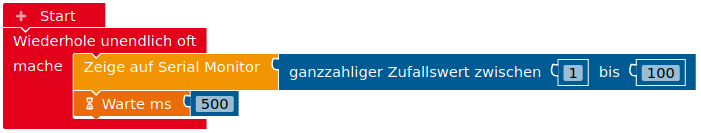
\includegraphics[width=0.5\textwidth]{pics/zufallszahlengenerator.png}
	\end{wrapfigure}
	Übertrage das rechts abgebildete Programm auf den Arduino und betrachte die so erzeugten Zufallszahlen. Drücke dann auf den Reset-Taster am Arduino und betrachte die nun erzeugten Zufallszahlen. Wiederhole den Vorgang einige Male und beschreibe Auffälligkeiten.
\end{aufgabe}

\newpage
\section{Kurze Einführung in die Codierung von Zahlen und Zeichen}
Wie wir gesehen haben, können der Computer und der Arduino nur die berühmten Einsen und Nullen austauschen.

\begin{ziel}
	\textbf{Frage:} Wie ist es möglich, mithilfe von Einsen und Nullen Zahlen und Zeichen darzustellen?
\end{ziel}

\subsection{Ein Einblick ins Binärsystem}\label{sec:binaer}

\begin{aufgabe}
	\begin{enumerate}[label=\alph*), noitemsep]
		\item Erkläre die unten dargestellte Zerlegung der Zahl 1509 im Dezimalsystem:
		\vspace{-0.5\baselineskip}
		\begin{align*}
		1509 &= 1\cdot 1000 + 5 \cdot 100 + 0\cdot 10 + 9 \cdot 1 \\
		&= 1\cdot 10^3+ 5\cdot 10^2 + 0 \cdot 10^1 + 9 \cdot 10^0
		\end{align*}
		\vspace{-1.5\baselineskip}
		\item Das Binärsystem arbeitet mit Zweierpotenzen statt Zehnerpotenzen. Notiere alle Zweierpotenzen von $2^0$ bis $2^{10}$. Erkläre kurz, wieso es bei der Verwendung von Zweierpotenzen nur die Ziffern $0$ und $1$ geben kann.
		\item Übersetze die Zahlen vom Binärsystem ins Dezimalsystem:
		\vspace{-0.5\baselineskip}
		\begin{multicols}{3}
			\begin{enumerate}[label=(\arabic*),noitemsep]
				\item 1011
				\item 11000001
				\item 01010101
			\end{enumerate}
		\end{multicols}
		\vspace{-0.5\baselineskip}
		\item Finde die Binär-Darstellungen von 12, 21 und 127.
		\item Ein Byte besteht aus acht Bit, also acht Nullen oder Einsen. Bestimme, wie viele verschiedene Zahlen man damit darstellen kann.
	\end{enumerate}
\end{aufgabe}

\marginpar{%
	\footnotesize%
	\werkzeug Neues \\
	Werkzeug:\\
	\hyperref[sec:lcd]{LC-Display}%
}
Für negative Zahlen und Zahlen mit Komma braucht man noch einige zusätzliche Kniffs, die an dieser Stelle zu weit führen.

\medskip
\begin{zsfg}{Das Binärsystem}
	
	Im Gegensatz zum Dezimalsystem zur Basis 10 mit Ziffern von 0 bis 9 arbeitet das Binärsystem zur Basis 2 mit den Ziffern 0 und 1.
	
	Im Binärsystem wird jede Zahl durch die Potenzen von 2 zusammengesetzt. Die Binärzahl \texttt{1001} bedeutet dann so viel wie $\texttt{1}\cdot 2^3 + \texttt{0}\cdot 2^2+ \texttt{0}\cdot 2^1 + \texttt{1}\cdot 2^0$. Den Wert der Binärzahl im Dezimalsystem erhält man dann durch eben diese Rechnung: $\texttt{1}\cdot 2^3 + \texttt{0}\cdot 2^2+ \texttt{0}\cdot 2^1 + \texttt{1}\cdot 2^0= 8 + 0 + 0 + 1 = 9$.
	
	Da bei Binärzahlen wie \texttt{1001} nicht sofort ersichtlich ist, ob es sich um eine Binärzahl oder eine Dezimalzahl handeln soll, wird der Zahl häufig ein \texttt{0b} vorangestellt: \texttt{0b1001}. Ebenfalls üblich ist es, die Basis im Index zu notieren: $\texttt{1001}_{2}$ zeigt eine Binärzahl an; $1001_{10}$ eine Dezimalzahl.
	
	Um die Binärdarstellung einer Dezimalzahl wie z.\,B. 13 zu finden, geht man folgendermaßen vor:
	
	\begin{minipage}{0.65\textwidth}
		\begin{enumerate}[noitemsep]
			\item Finde die größte Zweierpotenz, die in die Dezimalzahl passt. Notiere dafür eine \texttt{1}.
			\item Überprüfe, wie oft die nächstkleinere Zweierpotenz in den Rest passt. Notiere entsprechend eine \texttt{0} (passt nicht) oder eine \texttt{1} (passt einmal).
			\item Wiederhole den Schritt (2), bis kein Rest mehr übrig ist.
		\end{enumerate}
	\end{minipage}
	\hfill
	\begin{minipage}{0.34\textwidth}
		\begin{align*}
			13 &= 1\cdot 8 + 5 & \texttt{1~~~} \\
			5 &= 1\cdot 4 + 1 & \texttt{11~~} \\
			1 &= 0\cdot 2 +1 & \texttt{110~} \\
			1&= 1\cdot 1 & \texttt{1101} 
		\end{align*}
		\vspace{1\baselineskip}
	\end{minipage}
	\vspace{-\baselineskip}
\end{zsfg}

\subsection{Ein Einblick in die ASCII-Tabelle}
Auf diese Codierung im Binärsystem wird dann zurückgegriffen, wenn die übertragenen (bzw. abgespeicherten) Daten vom Typ \enquote{Zahl} sind. Wie man an der eckigen Form des Arguments im Block \button{Sende Text an seriellen Port} sieht, werden dabei aber Daten vom Typ \enquote{Zeichen} übertragen. Um welches Zeichen es sich handelt, lässt sich nicht allein anhand der Bits schlussfolgern, sondern muss durch einen Standard festgelegt werden. Der einfachste Standard ist der ASCII-Standard, der später in den Unicode- und schließlich in den UTF-8-Standard eingeflossen ist.

\begin{zsfg}{Der ASCII-Code}
	Der \href{http://www.computer-masters.de/ascii-tabelle.php}{American Standard Code for Information Interchange (ASCII)} legt durch eine Tabelle für 128 Zeichen fest, wie diese mithilfe von sieben Bits codiert werden. Wenn man diese Bitfolge nicht als Zeichen, sondern als Zahl interpretiert, kann man jedem Zeichen eine Zahl zuordnen, die diesem entspricht. Zum Beispiel wird der Buchstabe A durch die Folge 1000001 codiert und entspricht damit der Zahl 65.
\end{zsfg}

\begin{aufgabe}
	Finde und notiere die ASCII-Bitfolgen zu den Zeichen \enquote{V}, \enquote{s}, \enquote{+}, \enquote{?} und \enquote{0}.
	
	ASCII-Tabelle: \url{http://www.computer-masters.de/ascii-tabelle.php}
\end{aufgabe}

\begin{recherche}{Von ASCII über Unicode zu UTF-8}
	Der ASCII-Standard ist ausreichend, wenn man nur englische Texte darstellen muss. In anderen Sprachen ergibt sich jedoch die Herausforderung, weitere Zeichen codieren zu müssen und spätestens mit der Verbreitung des Internets und der weltweiten Kommunikation war das auch für englischsprachige Programmierer relevant. Eine locker geschriebene Einführung zur Entwicklung der unterschiedlichen Standards gibt der Artikel \href{https://www.joelonsoftware.com/2003/10/08/the-absolute-minimum-every-software-developer-absolutely-positively-must-know-about-unicode-and-character-sets-no-excuses/}{The Absolute Minimum Every Software Developer Absolutely, Positively Must Know About Unicode and Character Sets (No Excuses!)}.
	
	\emph{Hilfreich für das Verständnis des Artikels ist die Kenntnis von Hexadezimalzahlen (s. S. \pageref{proj:rgbled2} f.).}
\end{recherche}

\newpage
\section{Programme mit Struktogrammen darstellen}
Wenn wir uns über Programme austauschen, dann haben wir nicht immer den Computer zur Hand. In solchen Momenten wäre es viel zu aufwendig, die bunten Blöcke von mBlock zu malen. Außerdem könnte es sein, dass jemand anderes das Programm nicht mit Blöcken, sondern mit Text in der Programmiersprache C++ aufschreiben will, also so wie es in der rechten Seite von mBlock abgebildet ist.

\begin{ziel}
	\textbf{Frage:} Wie kann man Programme übersichtlich zu Papier bringen?
\end{ziel}

Man nutzt zur Darstellung des Ablaufs eines Computerprogramms sogenannte \textbf{Struktogramme} (vgl. Tab. \ref{tab:struktogramm}), die in den 1970er Jahren von Isaac Nassi und Ben Shneidermann entwickelt wurden. Struktogramme sollen ein Computerprogramm möglichst einfach und ohne programmiersprachenspezifische Befehlssyntax abbilden. Auf diese Art und Weise lassen sich Programme auch einfach planen, bevor man sich damit beschäftigt, wie die Schritte im Einzelnen zu codieren sind.

\begin{aufgabe}
	Stelle die unten abgebildeten Programme jeweils mithilfe eines Struktogramms dar. Fasse die Wirkung der Programme jeweils kurz zusammen.
\end{aufgabe}
\begin{figure}[H]
	\begin{minipage}{0.45\textwidth}
		\centering
		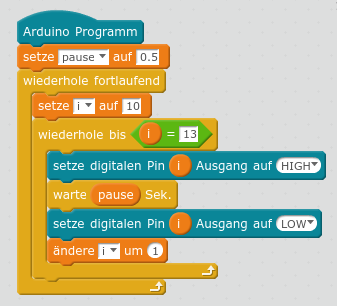
\includegraphics[width=0.9\textwidth]{./lsg/4-2-A1-Lauflicht-Lsg2.png}
		\caption{Programm A.}
	\end{minipage}
	\hfill
	\begin{minipage}{0.52\textwidth}
		\centering
		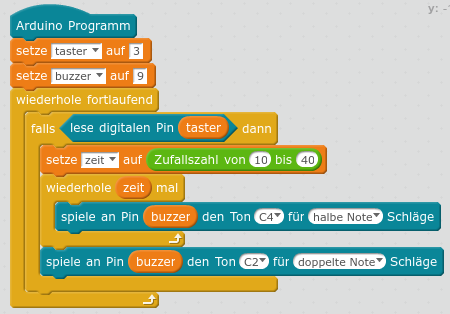
\includegraphics[width=\textwidth]{./lsg/4-3-Bombe-Lsg1.png}
		\caption{Programm B.}
	\end{minipage}
\end{figure}

\newpage

\begin{zsfg}{Darstellung von Programmen in Struktogrammen}
	
	\begin{table}[H]
   \centering
   \begin{minipage}[b]{\textwidth}
      \begin{tabu} to \textwidth {X[L,3]X[L,2]}
         \toprule
         \vspace{-4\baselineskip}
         \textbf{Lineare Struktur}
         
         Jede Anweisung wird in einen rechteckigen Block geschrieben.
          
         &
         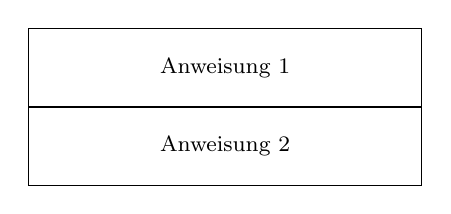
\begin{tikzpicture}
         	\draw (0,0) rectangle (5,1);
         	\node at (2.5,0.5) {\footnotesize Anweisung 2};
         	\draw (0,1) rectangle (5,2);
         	\node at (2.5,1.5) {\footnotesize Anweisung 1};
         \end{tikzpicture}
         \\
         \midrule%\hline
         %\rowcolor{CadetBlue!80!green}
         \textbf{Wiederholung / Schleifen} & \\
         \midrule%\hline
%         \vspace{-4.2\baselineskip}
		 \vspace{0mm}
         \textbf{Zählergesteuerte Schleife}
         
         Die Anzahl der Schleifendurchläufe wird durch eine Zählvariable festgelegt. Im Schleifenkopf werden der Startwert der Zählvariablen, der Endwert der Zählvariablen und die Veränderung der Zählvariablen, z.\,B. Schrittweite 1, angegeben.
         &
         \smallbreak
         \vspace{-0.7\baselineskip}
         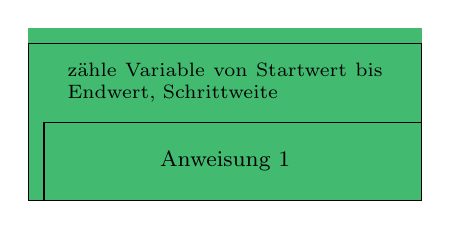
\begin{tikzpicture}
         	\fill [CadetBlue!70!green] (0,0) rectangle (5,2.2);
         	\draw (0,0) -- (0,2) -- (5,2) -- (5,1) -- (0.2,1) -- (0.2,0) -- (0,0);
         	\draw (0.2,0) -- (5,0) -- (5,1);
         	\node at (2.5,0.5) {\footnotesize Anweisung 1};
         	\node at (2.5,1.5) {\parbox{4cm}{\scriptsize zähle Variable von Startwert bis Endwert, Schrittweite}};
         \end{tikzpicture}
         \\
         \midrule
         \vspace{-4\baselineskip}
         \textbf{Kopfgesteuerte Schleife}
         
         Wiederholungsschleife mit vorausgehender Prüfung der Bedingung. Der Schleifenkörper wird so lange wiederholt, \emph{wie} oder \emph{bis} die Bedingung wahr ist (bei uns nur der letzte Fall verfügbar).
         &
         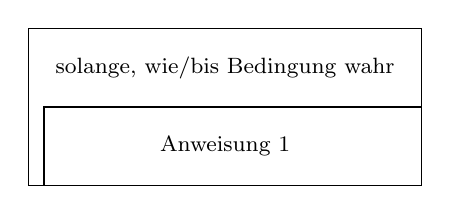
\begin{tikzpicture}
         \draw (0,0) -- (0,2) -- (5,2) -- (5,1) -- (0.2,1) -- (0.2,0) -- (0,0);
         \draw (0.2,0) -- (5,0) -- (5,1);
         \node at (2.5,0.5) {\footnotesize Anweisung 1};
         \node at (2.5,1.5) {\footnotesize solange, wie/bis Bedingung wahr};
         \end{tikzpicture}
         \\
         \midrule
         \vspace{-4\baselineskip}
         \textbf{Fußgesteuerte Schleife}
         
         Wiederholungsschleife mit nachfolgender Prüfung der Bedingung. Der Schleifenkörper wird so lange wiederholt, \emph{wie} oder \emph{bis} die Bedingung wahr ist (in mBlock nicht verfügbar).\smallskip
         &
         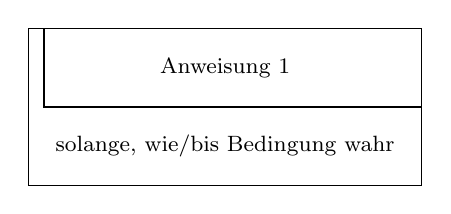
\begin{tikzpicture}
         \draw (0,0) -- (0,2) -- (0.2,2) -- (0.2,1) -- (5,1) -- (5,0) -- (0,0);
         \draw (0.2,2) -- (5,2) -- (5,1);
         \node at (2.5,1.5) {\footnotesize Anweisung 1};
         \node at (2.5,0.5) {\footnotesize solange, wie/bis Bedingung wahr};
         \end{tikzpicture}
         \\
         \midrule%\hline
         %\rowcolor{CadetBlue!80!green}
         \textbf{Verzweigung} & \\
         \midrule%\hline
         \vspace{0mm}
         \textbf{Einfache Verzweigung}
         
         Die Anweisung 1 (und ggf. weitere) wird nur ausgeführt, falls die Bedingung wahr ist. Andernfalls wird nichts gemacht.
         &
         \smallbreak
         \vspace{-0.7\baselineskip}
         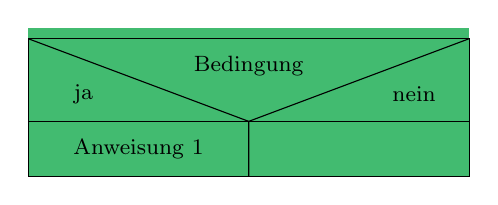
\begin{tikzpicture}[scale=0.7]
         \fill [CadetBlue!70!green] (0,0) rectangle (8,2.7);
         \draw (0,0) rectangle (8,2.5);
         \draw (0,1) -- (8,1);
         \draw (4,0) -- (4,1) -- (8,2.5);
         \draw (4,1) -- (0,2.5);
         \node at (2,0.5) {\footnotesize Anweisung 1};
         \node at (1,1.5) {\footnotesize ja};
         \node at (7,1.5) {\footnotesize nein};
         \node at (4,2) {\footnotesize Bedingung};
         \end{tikzpicture}
         \\
         \midrule
         \vspace{-3.5\baselineskip}
         \textbf{Alternative Verzweigung}
         
         Falls die Bedingung wahr ist, wird Anweisung 1 (und ggf. weitere) ausgeführt, sonst wird Anweisung 2 (und ggf. weitere) ausgeführt.
         &
         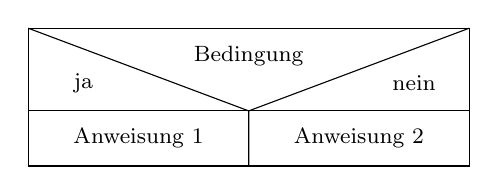
\begin{tikzpicture}[scale=0.7]
         \draw (0,0) rectangle (8,2.5);
         \draw (0,1) -- (8,1);
         \draw (4,0) -- (4,1) -- (8,2.5);
         \draw (4,1) -- (0,2.5);
         \node at (2,0.5) {\footnotesize Anweisung 1};
         \node at (6,0.5) {\footnotesize Anweisung 2};
         \node at (1,1.5) {\footnotesize ja};
         \node at (7,1.5) {\footnotesize nein};
         \node at (4,2) {\footnotesize Bedingung};
         \end{tikzpicture}
         \\
         \midrule
         \vspace{-5.5\baselineskip}
         \textbf{Verschachtelte Verzweigung}
         
         Falls Bedingung 1 wahr ist, folgt eine weitere Bedingung 2.
         &
         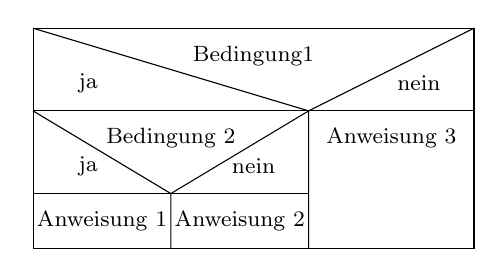
\begin{tikzpicture}[scale=0.7]
         \draw (0,-1.5) rectangle (8,2.5);
         \draw (0,1) -- (8,1);
         \draw (5,-1.5) -- (5,1) -- (8,2.5);
         \draw (5,1) -- (0,2.5);
         \draw (2.5,-1.5) -- (2.5,-0.5) -- (5,1);
         \draw (0,1) -- (2.5,-0.5);
         \draw (0,-0.5) -- (5,-0.5);
         \node at (1,1.5) {\footnotesize ja};
         \node at (7,1.5) {\footnotesize nein};
         \node at (4,2) {\footnotesize Bedingung1};
         \node at (1,0) {\footnotesize ja};
         \node at (4,0) {\footnotesize nein};
         \node at (2.5,0.5) {\footnotesize Bedingung 2};
         \node at (1.25,-1) {\footnotesize Anweisung 1};
         \node at (3.75,-1) {\footnotesize Anweisung 2};
         \node at (6.5,0.5) {\footnotesize Anweisung 3};
         \end{tikzpicture}
         \\
         \bottomrule
      \end{tabu}
   \end{minipage}
	\caption{Tabelle zur Darstellung eines Programms als Struktogramm nach Nassi und Shneidermann.}
   \label{tab:struktogramm}
\end{table}

\end{zsfg}

\section{Vermischte Übungen}

\begin{aufgabe} \emph{Variablen}
	\begin{enumerate}[label=\alph*),itemsep=0mm, parsep=0mm]
		\item Nenne Vorteile, die für die Verwendung von Variablen sprechen.
		\item Nenne drei Datentypen, die in Variablen abgespeichert werden können.
	\end{enumerate}
\end{aufgabe}

\begin{aufgabe} \emph{Schleifen}
	\medskip
	
	\begin{minipage}{0.6\textwidth}
		An allen Digitalpins des Arduino werden LEDs mit geeigneten Vorwiderständen angeschlossen. Dann wird das rechts abgebildete Programm ausgeführt.
		\begin{enumerate}[label=\alph*),itemsep=0mm, parsep=0mm]
			\item Erstelle eine Trace-Tabelle für einen Durchlauf der \button{Wiederhole fortlaufend}- Schleife.
			\item Nenne die Pin-Nummern der LEDs, die nach Durchlaufen dieses Programms einmal geleuchtet haben.
			\item Stelle das Programm als Struktogramm dar.
		\end{enumerate}
	\end{minipage}
	\hfill
	\begin{minipage}{0.38\textwidth}
		\centering
		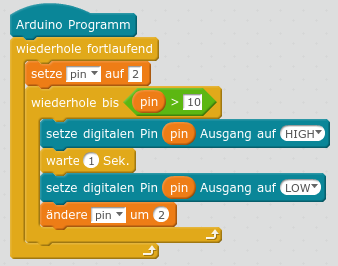
\includegraphics[width=\textwidth]{./pics/programm-trace-uebung.png}
	\end{minipage}
\end{aufgabe}

\bigskip
\begin{aufgabe} \emph{Bitübertragung}
	
	Ein Programm ist 30 kB groß. Berechne, wie lange es bei einer Bitrate von 115200 Bit pro Sekunde dauert, das Programm auf den Arduino zu übertragen.
\end{aufgabe}

\bigskip
\begin{aufgabe} \emph{Das Binärsystem und das Dezimalsystem}
	
	\begin{enumerate}[label=\alph*),itemsep=0mm, parsep=0mm]
		\item Übersetze vom Binär- ins Dezimalsystem.
		\begin{multicols}{3}
			\begin{enumerate}[label=(\arabic*)]
				\item $1001_2$
				\item $1010_2$
				\item $1111_2$
			\end{enumerate}
		\end{multicols}
		\item Übersetze vom Dezimal- ins Binärsystem.
		\begin{multicols}{3}
			\begin{enumerate}[label=(\arabic*)]
				\item 11
				\item 7
				\item 14
			\end{enumerate}
		\end{multicols}
	\end{enumerate}
\end{aufgabe}

\begin{aufgabe} \emph{Programme verstehen}
	
	\begin{minipage}{0.54\textwidth}
		Am Arduino wird an Pin 9 eine LED mit Vorwiderstand und an Pin 10 ein Piezo-Summer angebracht.
		\begin{enumerate}[label=\alph*),itemsep=0mm, parsep=0mm]
			\item Stelle das Programm als Struktogramm dar.
			\item Beschreibe die Wirkung des rechts abgebildeten Programms.
			\item Erkläre, wie man das Programm ändern müsste, damit die LED zwei Mal blinkt, bevor wieder der Piezo-Summer piept.
		\end{enumerate}
		\vspace{2\baselineskip}
	\end{minipage}
	\hfill
	\begin{minipage}{0.45\textwidth}
		\centering
		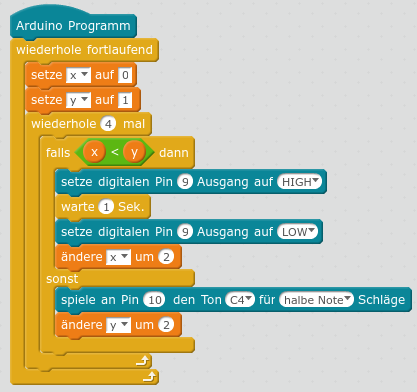
\includegraphics[width=\textwidth]{./pics/Uebung-Variablen-und-Schleifen.png}
	\end{minipage}
\end{aufgabe}

\begin{aufgabe} \emph{Programm entwickeln}
	
	An allen Digitalpins des Arduino sind LEDs mit Vorwiderstand angeschlossen.	Für das folgende Programm ist bereits eine Variable namens \button{p} angelegt. 
	
	Entwickle ein Programm, das die LEDs an Pin 1 bis 5 [2,4,6,8] nacheinander zum Leuchten bringt und nach einer Sekunde wieder ausschaltet. Es leuchtet also immer nur eine LED zur selben Zeit. 
	
	\medskip
	\emph{Anforderungen:}
	\begin{itemize}[noitemsep]
		\item Das Programm soll als Struktogramm dargestellt werden.
		\item Es sollen so wenig Code-Wiederholungen wie möglich vorkommen (\emph{effizientes Programmieren}).
	\end{itemize}
		
	\emph{Befehle:}
	\begin{figure}[H]
		\centering
		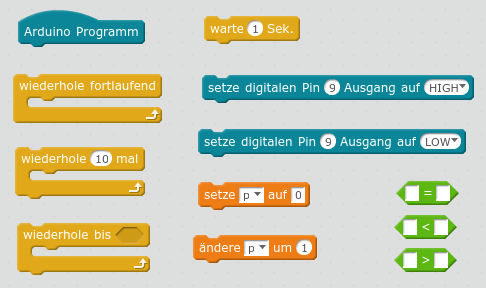
\includegraphics[width=0.6\textwidth]{./pics/Uebung-Programm-entwickeln-Befehlssammlung.png}
	\end{figure}
\end{aufgabe}

\vfill
\begin{links}
	\item \href{https://www.heise.de/make/meldung/Schueler-Projekt-Selbstbau-Staubsaugerroboter-aus-dem-3D-Drucker-3991208.html}{Staubsaugerroboter}
	
	Mithilfe eines Arduino haben zwei Schüler aus den Niederlanden ihren eigenen Staubsaugerroboter gebaut. Das Teile für das Gehäuse haben sie mit einem 3D-Drucker gedruckt.
	
	\item \href{https://www.heise.de/make/artikel/Einfacher-Ultraschall-Levitationsapparat-4022505.html}{Levitation}
	
	Durch Levitation lassen sich Gegenstände scheinbar von Geisterhand in der Luft schweben. Die nötige Elektronik dafür lässt sich mit einem Arduino realisieren.
	
	\item \href{https://www.instructables.com/id/Party-Lights-1/}{Arduino-kontrollierter LED-Streifen zur Visualisierung von Musik}
	
	Der Arduino lässt sich zudem über ein Smartphone ansteuern.
	
	\item \href{https://www.heise.de/make/meldung/Makerbuino-Spielkonsole-fuer-den-Eigenbau-3681578.html}{Spielekonsole von Makerbuino}
	
	Mithilfe eines Bausatzes lässt sich eine kleine, Arduino-basierte Spielekonsole bauen.
\end{links}

